\documentclass[twoside]{book}

% Packages required by doxygen
\usepackage{fixltx2e}
\usepackage{calc}
\usepackage{doxygen}
\usepackage[export]{adjustbox} % also loads graphicx
\usepackage{graphicx}
\usepackage[utf8]{inputenc}
\usepackage{makeidx}
\usepackage{multicol}
\usepackage{multirow}
\PassOptionsToPackage{warn}{textcomp}
\usepackage{textcomp}
\usepackage[nointegrals]{wasysym}
\usepackage[table]{xcolor}

% Font selection
\usepackage[T1]{fontenc}
\usepackage[scaled=.90]{helvet}
\usepackage{courier}
\usepackage{amssymb}
\usepackage{sectsty}
\renewcommand{\familydefault}{\sfdefault}
\allsectionsfont{%
  \fontseries{bc}\selectfont%
  \color{darkgray}%
}
\renewcommand{\DoxyLabelFont}{%
  \fontseries{bc}\selectfont%
  \color{darkgray}%
}
\newcommand{\+}{\discretionary{\mbox{\scriptsize$\hookleftarrow$}}{}{}}

% Page & text layout
\usepackage{geometry}
\geometry{%
  a4paper,%
  top=2.5cm,%
  bottom=2.5cm,%
  left=2.5cm,%
  right=2.5cm%
}
\tolerance=750
\hfuzz=15pt
\hbadness=750
\setlength{\emergencystretch}{15pt}
\setlength{\parindent}{0cm}
\setlength{\parskip}{3ex plus 2ex minus 2ex}
\makeatletter
\renewcommand{\paragraph}{%
  \@startsection{paragraph}{4}{0ex}{-1.0ex}{1.0ex}{%
    \normalfont\normalsize\bfseries\SS@parafont%
  }%
}
\renewcommand{\subparagraph}{%
  \@startsection{subparagraph}{5}{0ex}{-1.0ex}{1.0ex}{%
    \normalfont\normalsize\bfseries\SS@subparafont%
  }%
}
\makeatother

% Headers & footers
\usepackage{fancyhdr}
\pagestyle{fancyplain}
\fancyhead[LE]{\fancyplain{}{\bfseries\thepage}}
\fancyhead[CE]{\fancyplain{}{}}
\fancyhead[RE]{\fancyplain{}{\bfseries\leftmark}}
\fancyhead[LO]{\fancyplain{}{\bfseries\rightmark}}
\fancyhead[CO]{\fancyplain{}{}}
\fancyhead[RO]{\fancyplain{}{\bfseries\thepage}}
\fancyfoot[LE]{\fancyplain{}{}}
\fancyfoot[CE]{\fancyplain{}{}}
\fancyfoot[RE]{\fancyplain{}{\bfseries\scriptsize Generated by Doxygen }}
\fancyfoot[LO]{\fancyplain{}{\bfseries\scriptsize Generated by Doxygen }}
\fancyfoot[CO]{\fancyplain{}{}}
\fancyfoot[RO]{\fancyplain{}{}}
\renewcommand{\footrulewidth}{0.4pt}
\renewcommand{\chaptermark}[1]{%
  \markboth{#1}{}%
}
\renewcommand{\sectionmark}[1]{%
  \markright{\thesection\ #1}%
}

% Indices & bibliography
\usepackage{natbib}
\usepackage[titles]{tocloft}
\setcounter{tocdepth}{3}
\setcounter{secnumdepth}{5}
\makeindex

% Hyperlinks (required, but should be loaded last)
\usepackage{ifpdf}
\ifpdf
  \usepackage[pdftex,pagebackref=true]{hyperref}
\else
  \usepackage[ps2pdf,pagebackref=true]{hyperref}
\fi
\hypersetup{%
  colorlinks=true,%
  linkcolor=blue,%
  citecolor=blue,%
  unicode%
}

% Custom commands
\newcommand{\clearemptydoublepage}{%
  \newpage{\pagestyle{empty}\cleardoublepage}%
}

\usepackage{caption}
\captionsetup{labelsep=space,justification=centering,font={bf},singlelinecheck=off,skip=4pt,position=top}

%===== C O N T E N T S =====

\begin{document}

% Titlepage & ToC
\hypersetup{pageanchor=false,
             bookmarksnumbered=true,
             pdfencoding=unicode
            }
\pagenumbering{alph}
\begin{titlepage}
\vspace*{7cm}
\begin{center}%
{\Large Brachytherapy }\\
\vspace*{1cm}
{\large Generated by Doxygen 1.8.14}\\
\end{center}
\end{titlepage}
\clearemptydoublepage
\pagenumbering{roman}
\tableofcontents
\clearemptydoublepage
\pagenumbering{arabic}
\hypersetup{pageanchor=true}

%--- Begin generated contents ---
\chapter{Hierarchical Index}
\section{Class Hierarchy}
This inheritance list is sorted roughly, but not completely, alphabetically\+:\begin{DoxyCompactList}
\item Mono\+Behaviour\begin{DoxyCompactList}
\item \contentsline{section}{Needle\+Controller}{\pageref{class_needle_controller}}{}
\item \contentsline{section}{States\+By\+Switch}{\pageref{class_states_by_switch}}{}
\end{DoxyCompactList}
\end{DoxyCompactList}

\chapter{Class Index}
\section{Class List}
Here are the classes, structs, unions and interfaces with brief descriptions\+:\begin{DoxyCompactList}
\item\contentsline{section}{\mbox{\hyperlink{class_needle_controller}{Needle\+Controller}} \\*Handles the movement of the needles }{\pageref{class_needle_controller}}{}
\item\contentsline{section}{\mbox{\hyperlink{class_states_by_switch}{States\+By\+Switch}} \\*Guides the player through the planning steps of the Simulation }{\pageref{class_states_by_switch}}{}
\end{DoxyCompactList}

\chapter{Class Documentation}
\hypertarget{class_needle_controller}{}\section{Needle\+Controller Class Reference}
\label{class_needle_controller}\index{Needle\+Controller@{Needle\+Controller}}


Handles the movement of the needles.  


Inheritance diagram for Needle\+Controller\+:\begin{figure}[H]
\begin{center}
\leavevmode
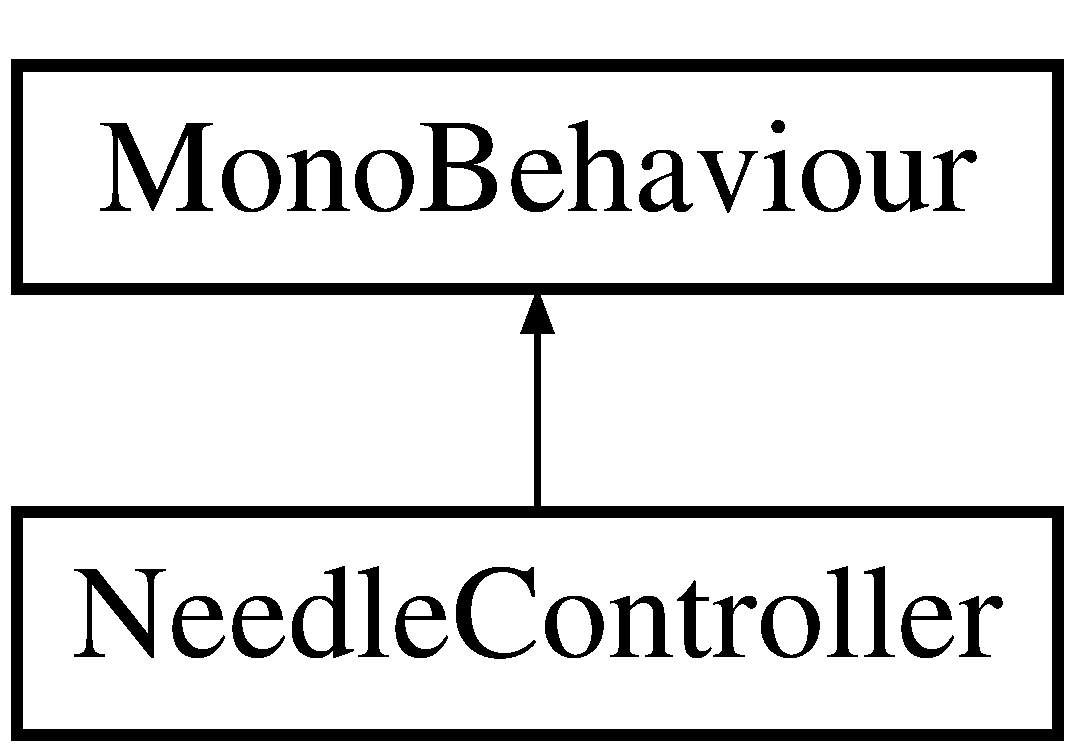
\includegraphics[height=2.000000cm]{class_needle_controller}
\end{center}
\end{figure}
\subsection*{Public Attributes}
\begin{DoxyCompactItemize}
\item 
\mbox{\Hypertarget{class_needle_controller_a34e6c905f03f3bb0afb22a60ca868913}\label{class_needle_controller_a34e6c905f03f3bb0afb22a60ca868913}} 
float \mbox{\hyperlink{class_needle_controller_a34e6c905f03f3bb0afb22a60ca868913}{speed}}
\begin{DoxyCompactList}\small\item\em Adjustement of the forward/backward movement of the needle. \end{DoxyCompactList}\item 
\mbox{\Hypertarget{class_needle_controller_a095ef158c2feb66537428d385bcddebc}\label{class_needle_controller_a095ef158c2feb66537428d385bcddebc}} 
Game\+Object \mbox{\hyperlink{class_needle_controller_a095ef158c2feb66537428d385bcddebc}{Seed}}
\begin{DoxyCompactList}\small\item\em The Seed planted in the Tumor. \end{DoxyCompactList}\item 
\mbox{\Hypertarget{class_needle_controller_a8a35d1e5d95210f8be9a00fe9437ae0b}\label{class_needle_controller_a8a35d1e5d95210f8be9a00fe9437ae0b}} 
Slider \mbox{\hyperlink{class_needle_controller_a8a35d1e5d95210f8be9a00fe9437ae0b}{Speed\+Slider}}
\begin{DoxyCompactList}\small\item\em The adjustable Slider in the top right of the game screen. \end{DoxyCompactList}\end{DoxyCompactItemize}
\subsection*{Private Member Functions}
\begin{DoxyCompactItemize}
\item 
void \mbox{\hyperlink{class_needle_controller_a273d374ac8d5504706fc431af48b91cc}{Update}} ()
\end{DoxyCompactItemize}


\subsection{Detailed Description}
Handles the movement of the needles. 

\subsection{Member Function Documentation}
\mbox{\Hypertarget{class_needle_controller_a273d374ac8d5504706fc431af48b91cc}\label{class_needle_controller_a273d374ac8d5504706fc431af48b91cc}} 
\index{Needle\+Controller@{Needle\+Controller}!Update@{Update}}
\index{Update@{Update}!Needle\+Controller@{Needle\+Controller}}
\subsubsection{\texorpdfstring{Update()}{Update()}}
{\footnotesize\ttfamily void Needle\+Controller.\+Update (\begin{DoxyParamCaption}{ }\end{DoxyParamCaption})\hspace{0.3cm}{\ttfamily [private]}}

$<$ Movement of the Needle, vertical and horizontal The forward and backward movement speed can be adjusted through the variable \textquotesingle{}speed\textquotesingle{} Includes the feature of \char`\"{}planting\char`\"{} the seed 

The documentation for this class was generated from the following file\+:\begin{DoxyCompactItemize}
\item 
C\+:/\+Users/\+Faiq Bakar/\+Bachelorstuff/\+Asset Tests/\+Assets/\+Scripts/Needle\+Controller.\+cs\end{DoxyCompactItemize}

\hypertarget{class_states_by_switch}{}\section{States\+By\+Switch Class Reference}
\label{class_states_by_switch}\index{States\+By\+Switch@{States\+By\+Switch}}


Guides the player through the planning steps of the Simulation  


Inheritance diagram for States\+By\+Switch\+:\begin{figure}[H]
\begin{center}
\leavevmode
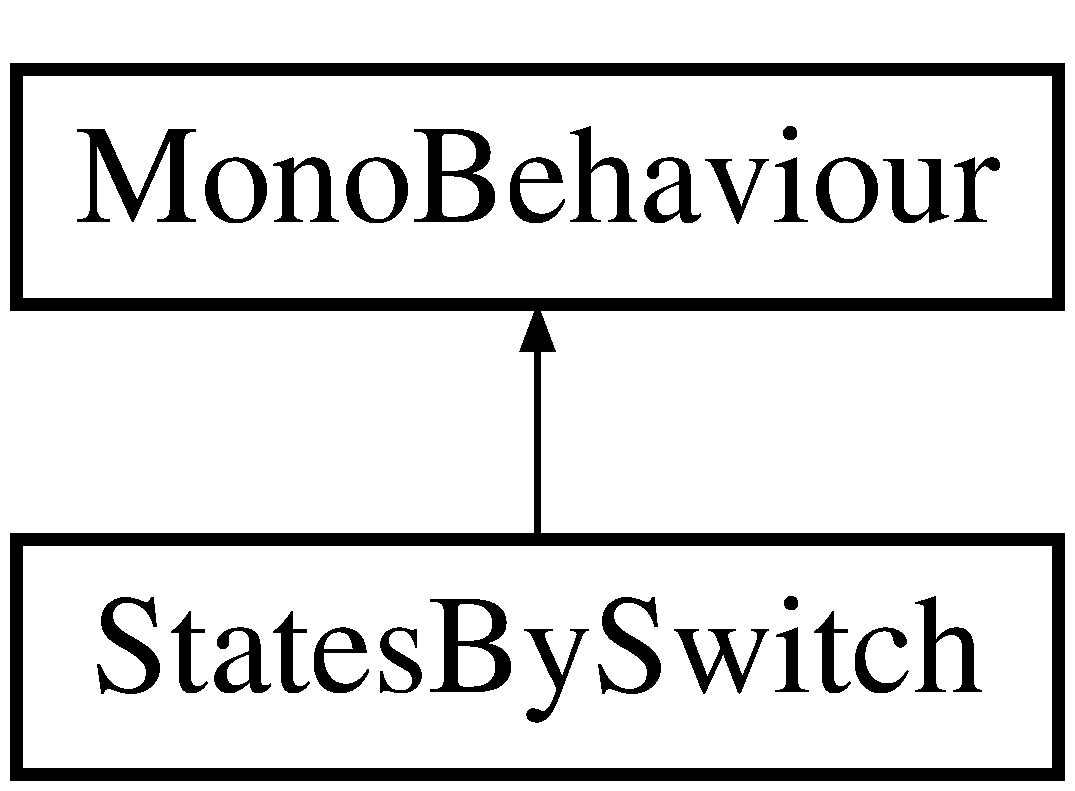
\includegraphics[height=2.000000cm]{class_states_by_switch}
\end{center}
\end{figure}
\subsection*{Public Member Functions}
\begin{DoxyCompactItemize}
\item 
void \mbox{\hyperlink{class_states_by_switch_a21dce0c656d329bd4890e0ec07c6b8c9}{Start}} ()
\begin{DoxyCompactList}\small\item\em Toggles the texts inactive and enters the first phase \end{DoxyCompactList}\end{DoxyCompactItemize}
\subsection*{Public Attributes}
\begin{DoxyCompactItemize}
\item 
Game\+Object \mbox{\hyperlink{class_states_by_switch_ac45169b7b1eeeeec3983d4c9109fb144}{needle}}
\item 
Transform \mbox{\hyperlink{class_states_by_switch_a22ee2b11d00f659a78da32cec049de22}{tumor}}
\item 
\mbox{\Hypertarget{class_states_by_switch_a3f091084e5763ac5398db2e400b3e4db}\label{class_states_by_switch_a3f091084e5763ac5398db2e400b3e4db}} 
Transform \mbox{\hyperlink{class_states_by_switch_a3f091084e5763ac5398db2e400b3e4db}{Fix\+Point}}
\begin{DoxyCompactList}\small\item\em Object in World Space to fixate one the two endpoints of the cameras to, to make it more accurate. \end{DoxyCompactList}\item 
Game\+Object \mbox{\hyperlink{class_states_by_switch_a6350a4b4edd29eab4d2f1a00ce3890dd}{Marker}}
\item 
Game\+Object \mbox{\hyperlink{class_states_by_switch_a3b340adadbafc43f0679c3270fb84a07}{Cylinder}}
\item 
Camera \mbox{\hyperlink{class_states_by_switch_aa48de7de6af496872584ba82e82b20eb}{Cam1}}
\item 
Text \mbox{\hyperlink{class_states_by_switch_ac7c8a7d50ecf021994bc930d51cbccb2}{Planning\+\_\+\+Text}}
\begin{DoxyCompactList}\small\item\em Helping text of the planning phase \end{DoxyCompactList}\item 
Text \mbox{\hyperlink{class_states_by_switch_a010d70d2a27cdd261b50ad93dfa4c6d4}{Marking\+\_\+\+Text}}
\begin{DoxyCompactList}\small\item\em Helping text of the Marking phase \end{DoxyCompactList}\item 
Text \mbox{\hyperlink{class_states_by_switch_a46b23045719e76ba9455fa84d2c4613a}{Introduction\+\_\+\+Text}}
\begin{DoxyCompactList}\small\item\em Helping text for the beginning of the actual game after the States phase \end{DoxyCompactList}\item 
Text \mbox{\hyperlink{class_states_by_switch_a36ebc107be9b12cb8a97bf1460423000}{Needle\+\_\+\+Placement\+\_\+\+Text}}
\begin{DoxyCompactList}\small\item\em Helping text of needle placement phase \end{DoxyCompactList}\item 
Game\+Object \mbox{\hyperlink{class_states_by_switch_a2a073b0e193c0609b5c3681434b4f24e}{Camera\+Skin\+Point}}
\item 
Needle\+Movement \mbox{\hyperlink{class_states_by_switch_a6b08cab5dde267f953387e4885318be4}{ascript}}
\begin{DoxyCompactList}\small\item\em Script that gets disabled during this script \end{DoxyCompactList}\end{DoxyCompactItemize}
\subsection*{Private Member Functions}
\begin{DoxyCompactItemize}
\item 
I\+Enumerator \mbox{\hyperlink{class_states_by_switch_abdcace6428d6394da78e41b19483e813}{Co\+Update}} ()
\begin{DoxyCompactList}\small\item\em Necessary function for routine delay for the text at the final stage \end{DoxyCompactList}\item 
void \mbox{\hyperlink{class_states_by_switch_adb2e0b871f32a901e5a9a4554cd3f797}{Update}} ()
\begin{DoxyCompactList}\small\item\em Handles all the phases \end{DoxyCompactList}\end{DoxyCompactItemize}
\subsection*{Private Attributes}
\begin{DoxyCompactItemize}
\item 
Raycast\+Hit \mbox{\hyperlink{class_states_by_switch_a541dfd2e3ba0cdfa1a33656455a2086f}{hit}}
\item 
State\+Ids \mbox{\hyperlink{class_states_by_switch_a6c039db026faf623438de4774163cf64}{current\+State\+Id}}
\begin{DoxyCompactList}\small\item\em Handles the current states \end{DoxyCompactList}\end{DoxyCompactItemize}


\subsection{Detailed Description}
Guides the player through the planning steps of the Simulation 



\subsection{Member Function Documentation}
\mbox{\Hypertarget{class_states_by_switch_abdcace6428d6394da78e41b19483e813}\label{class_states_by_switch_abdcace6428d6394da78e41b19483e813}} 
\index{States\+By\+Switch@{States\+By\+Switch}!Co\+Update@{Co\+Update}}
\index{Co\+Update@{Co\+Update}!States\+By\+Switch@{States\+By\+Switch}}
\subsubsection{\texorpdfstring{Co\+Update()}{CoUpdate()}}
{\footnotesize\ttfamily I\+Enumerator States\+By\+Switch.\+Co\+Update (\begin{DoxyParamCaption}{ }\end{DoxyParamCaption})\hspace{0.3cm}{\ttfamily [private]}}



Necessary function for routine delay for the text at the final stage 

\begin{DoxyReturn}{Returns}

\end{DoxyReturn}
\mbox{\Hypertarget{class_states_by_switch_a21dce0c656d329bd4890e0ec07c6b8c9}\label{class_states_by_switch_a21dce0c656d329bd4890e0ec07c6b8c9}} 
\index{States\+By\+Switch@{States\+By\+Switch}!Start@{Start}}
\index{Start@{Start}!States\+By\+Switch@{States\+By\+Switch}}
\subsubsection{\texorpdfstring{Start()}{Start()}}
{\footnotesize\ttfamily void States\+By\+Switch.\+Start (\begin{DoxyParamCaption}{ }\end{DoxyParamCaption})}



Toggles the texts inactive and enters the first phase 

\mbox{\Hypertarget{class_states_by_switch_adb2e0b871f32a901e5a9a4554cd3f797}\label{class_states_by_switch_adb2e0b871f32a901e5a9a4554cd3f797}} 
\index{States\+By\+Switch@{States\+By\+Switch}!Update@{Update}}
\index{Update@{Update}!States\+By\+Switch@{States\+By\+Switch}}
\subsubsection{\texorpdfstring{Update()}{Update()}}
{\footnotesize\ttfamily void States\+By\+Switch.\+Update (\begin{DoxyParamCaption}{ }\end{DoxyParamCaption})\hspace{0.3cm}{\ttfamily [private]}}



Handles all the phases 



\subsection{Member Data Documentation}
\mbox{\Hypertarget{class_states_by_switch_a6b08cab5dde267f953387e4885318be4}\label{class_states_by_switch_a6b08cab5dde267f953387e4885318be4}} 
\index{States\+By\+Switch@{States\+By\+Switch}!ascript@{ascript}}
\index{ascript@{ascript}!States\+By\+Switch@{States\+By\+Switch}}
\subsubsection{\texorpdfstring{ascript}{ascript}}
{\footnotesize\ttfamily Needle\+Movement States\+By\+Switch.\+ascript}



Script that gets disabled during this script 

\mbox{\Hypertarget{class_states_by_switch_aa48de7de6af496872584ba82e82b20eb}\label{class_states_by_switch_aa48de7de6af496872584ba82e82b20eb}} 
\index{States\+By\+Switch@{States\+By\+Switch}!Cam1@{Cam1}}
\index{Cam1@{Cam1}!States\+By\+Switch@{States\+By\+Switch}}
\subsubsection{\texorpdfstring{Cam1}{Cam1}}
{\footnotesize\ttfamily Camera States\+By\+Switch.\+Cam1}





\mbox{\Hypertarget{class_states_by_switch_a2a073b0e193c0609b5c3681434b4f24e}\label{class_states_by_switch_a2a073b0e193c0609b5c3681434b4f24e}} 
\index{States\+By\+Switch@{States\+By\+Switch}!Camera\+Skin\+Point@{Camera\+Skin\+Point}}
\index{Camera\+Skin\+Point@{Camera\+Skin\+Point}!States\+By\+Switch@{States\+By\+Switch}}
\subsubsection{\texorpdfstring{Camera\+Skin\+Point}{CameraSkinPoint}}
{\footnotesize\ttfamily Game\+Object States\+By\+Switch.\+Camera\+Skin\+Point}





\mbox{\Hypertarget{class_states_by_switch_a6c039db026faf623438de4774163cf64}\label{class_states_by_switch_a6c039db026faf623438de4774163cf64}} 
\index{States\+By\+Switch@{States\+By\+Switch}!current\+State\+Id@{current\+State\+Id}}
\index{current\+State\+Id@{current\+State\+Id}!States\+By\+Switch@{States\+By\+Switch}}
\subsubsection{\texorpdfstring{current\+State\+Id}{currentStateId}}
{\footnotesize\ttfamily State\+Ids States\+By\+Switch.\+current\+State\+Id\hspace{0.3cm}{\ttfamily [private]}}



Handles the current states 

\mbox{\Hypertarget{class_states_by_switch_a3b340adadbafc43f0679c3270fb84a07}\label{class_states_by_switch_a3b340adadbafc43f0679c3270fb84a07}} 
\index{States\+By\+Switch@{States\+By\+Switch}!Cylinder@{Cylinder}}
\index{Cylinder@{Cylinder}!States\+By\+Switch@{States\+By\+Switch}}
\subsubsection{\texorpdfstring{Cylinder}{Cylinder}}
{\footnotesize\ttfamily Game\+Object States\+By\+Switch.\+Cylinder}





\mbox{\Hypertarget{class_states_by_switch_a541dfd2e3ba0cdfa1a33656455a2086f}\label{class_states_by_switch_a541dfd2e3ba0cdfa1a33656455a2086f}} 
\index{States\+By\+Switch@{States\+By\+Switch}!hit@{hit}}
\index{hit@{hit}!States\+By\+Switch@{States\+By\+Switch}}
\subsubsection{\texorpdfstring{hit}{hit}}
{\footnotesize\ttfamily Raycast\+Hit States\+By\+Switch.\+hit\hspace{0.3cm}{\ttfamily [private]}}





\mbox{\Hypertarget{class_states_by_switch_a46b23045719e76ba9455fa84d2c4613a}\label{class_states_by_switch_a46b23045719e76ba9455fa84d2c4613a}} 
\index{States\+By\+Switch@{States\+By\+Switch}!Introduction\+\_\+\+Text@{Introduction\+\_\+\+Text}}
\index{Introduction\+\_\+\+Text@{Introduction\+\_\+\+Text}!States\+By\+Switch@{States\+By\+Switch}}
\subsubsection{\texorpdfstring{Introduction\+\_\+\+Text}{Introduction\_Text}}
{\footnotesize\ttfamily Text States\+By\+Switch.\+Introduction\+\_\+\+Text}



Helping text for the beginning of the actual game after the States phase 

\mbox{\Hypertarget{class_states_by_switch_a6350a4b4edd29eab4d2f1a00ce3890dd}\label{class_states_by_switch_a6350a4b4edd29eab4d2f1a00ce3890dd}} 
\index{States\+By\+Switch@{States\+By\+Switch}!Marker@{Marker}}
\index{Marker@{Marker}!States\+By\+Switch@{States\+By\+Switch}}
\subsubsection{\texorpdfstring{Marker}{Marker}}
{\footnotesize\ttfamily Game\+Object States\+By\+Switch.\+Marker}





\mbox{\Hypertarget{class_states_by_switch_a010d70d2a27cdd261b50ad93dfa4c6d4}\label{class_states_by_switch_a010d70d2a27cdd261b50ad93dfa4c6d4}} 
\index{States\+By\+Switch@{States\+By\+Switch}!Marking\+\_\+\+Text@{Marking\+\_\+\+Text}}
\index{Marking\+\_\+\+Text@{Marking\+\_\+\+Text}!States\+By\+Switch@{States\+By\+Switch}}
\subsubsection{\texorpdfstring{Marking\+\_\+\+Text}{Marking\_Text}}
{\footnotesize\ttfamily Text States\+By\+Switch.\+Marking\+\_\+\+Text}



Helping text of the Marking phase 

\mbox{\Hypertarget{class_states_by_switch_ac45169b7b1eeeeec3983d4c9109fb144}\label{class_states_by_switch_ac45169b7b1eeeeec3983d4c9109fb144}} 
\index{States\+By\+Switch@{States\+By\+Switch}!needle@{needle}}
\index{needle@{needle}!States\+By\+Switch@{States\+By\+Switch}}
\subsubsection{\texorpdfstring{needle}{needle}}
{\footnotesize\ttfamily Game\+Object States\+By\+Switch.\+needle}





\mbox{\Hypertarget{class_states_by_switch_a36ebc107be9b12cb8a97bf1460423000}\label{class_states_by_switch_a36ebc107be9b12cb8a97bf1460423000}} 
\index{States\+By\+Switch@{States\+By\+Switch}!Needle\+\_\+\+Placement\+\_\+\+Text@{Needle\+\_\+\+Placement\+\_\+\+Text}}
\index{Needle\+\_\+\+Placement\+\_\+\+Text@{Needle\+\_\+\+Placement\+\_\+\+Text}!States\+By\+Switch@{States\+By\+Switch}}
\subsubsection{\texorpdfstring{Needle\+\_\+\+Placement\+\_\+\+Text}{Needle\_Placement\_Text}}
{\footnotesize\ttfamily Text States\+By\+Switch.\+Needle\+\_\+\+Placement\+\_\+\+Text}



Helping text of needle placement phase 

\mbox{\Hypertarget{class_states_by_switch_ac7c8a7d50ecf021994bc930d51cbccb2}\label{class_states_by_switch_ac7c8a7d50ecf021994bc930d51cbccb2}} 
\index{States\+By\+Switch@{States\+By\+Switch}!Planning\+\_\+\+Text@{Planning\+\_\+\+Text}}
\index{Planning\+\_\+\+Text@{Planning\+\_\+\+Text}!States\+By\+Switch@{States\+By\+Switch}}
\subsubsection{\texorpdfstring{Planning\+\_\+\+Text}{Planning\_Text}}
{\footnotesize\ttfamily Text States\+By\+Switch.\+Planning\+\_\+\+Text}



Helping text of the planning phase 

\mbox{\Hypertarget{class_states_by_switch_a22ee2b11d00f659a78da32cec049de22}\label{class_states_by_switch_a22ee2b11d00f659a78da32cec049de22}} 
\index{States\+By\+Switch@{States\+By\+Switch}!tumor@{tumor}}
\index{tumor@{tumor}!States\+By\+Switch@{States\+By\+Switch}}
\subsubsection{\texorpdfstring{tumor}{tumor}}
{\footnotesize\ttfamily Transform States\+By\+Switch.\+tumor}







The documentation for this class was generated from the following file\+:\begin{DoxyCompactItemize}
\item 
C\+:/\+Users/\+Faiq Bakar/\+Bachelorstuff/\+Asset Tests/\+Assets/\+Scripts/States\+By\+Switch.\+cs\end{DoxyCompactItemize}

%--- End generated contents ---

% Index
\backmatter
\newpage
\phantomsection
\clearemptydoublepage
\addcontentsline{toc}{chapter}{Index}
\printindex

\end{document}
